\begin{figure*}
\centering
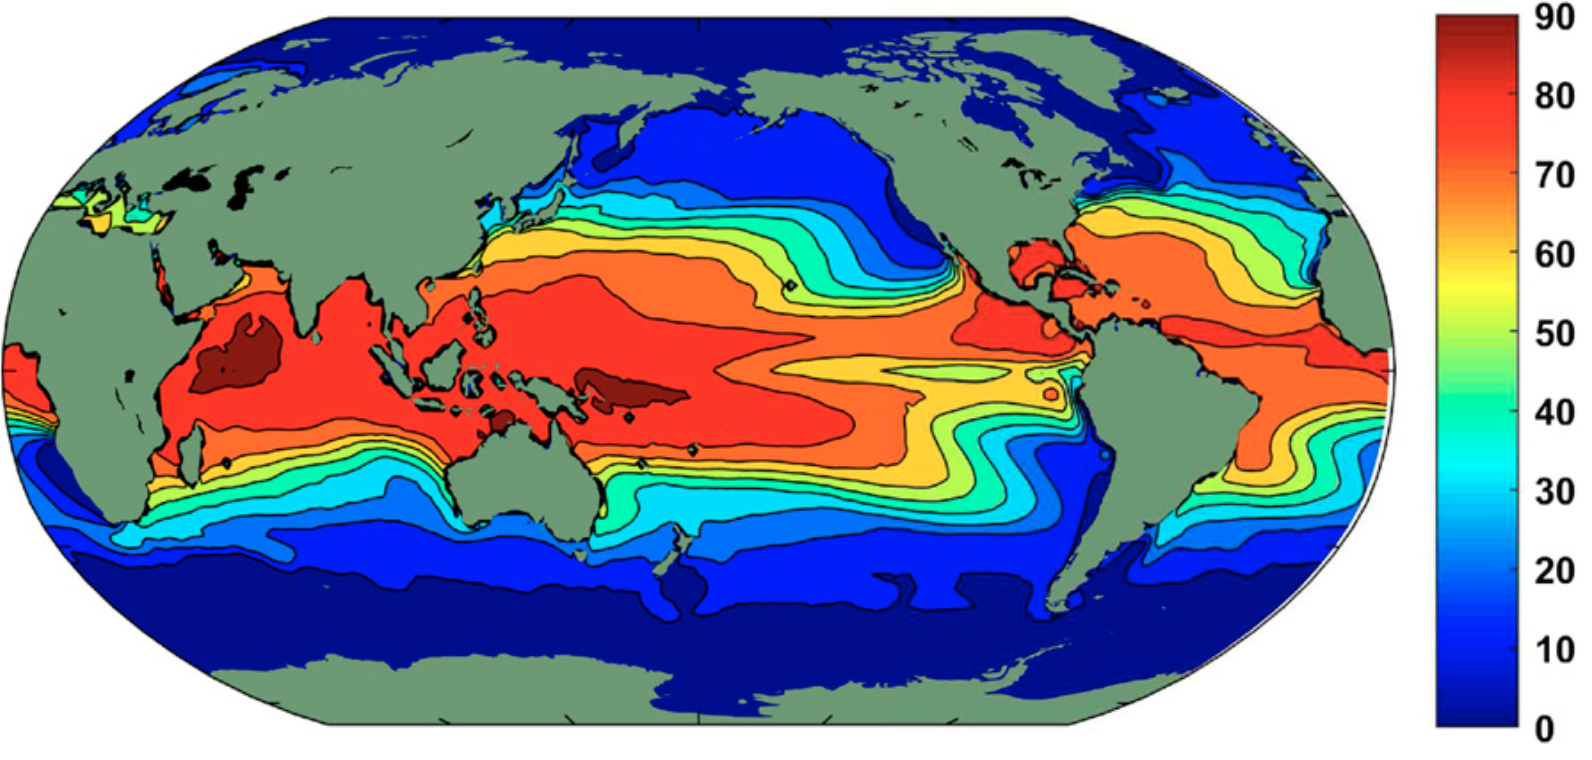
\includegraphics[width=\linewidth]{images/PI-max-year.png}\\
\textit{Figure 15-7 from \cite{emanuel2018progress}.}
\caption{The annual maximum of the potential intensity (m s$^{-1}$), calculated using
the algorithm from~\cite{bister2002low} and ERA-Interim data 1979-2016~\cite{berrisford2009era}.
This is product maps on well to the block maxima procedure in §~\ref{sec:evt}.
}
\label{fig:eman-pi}
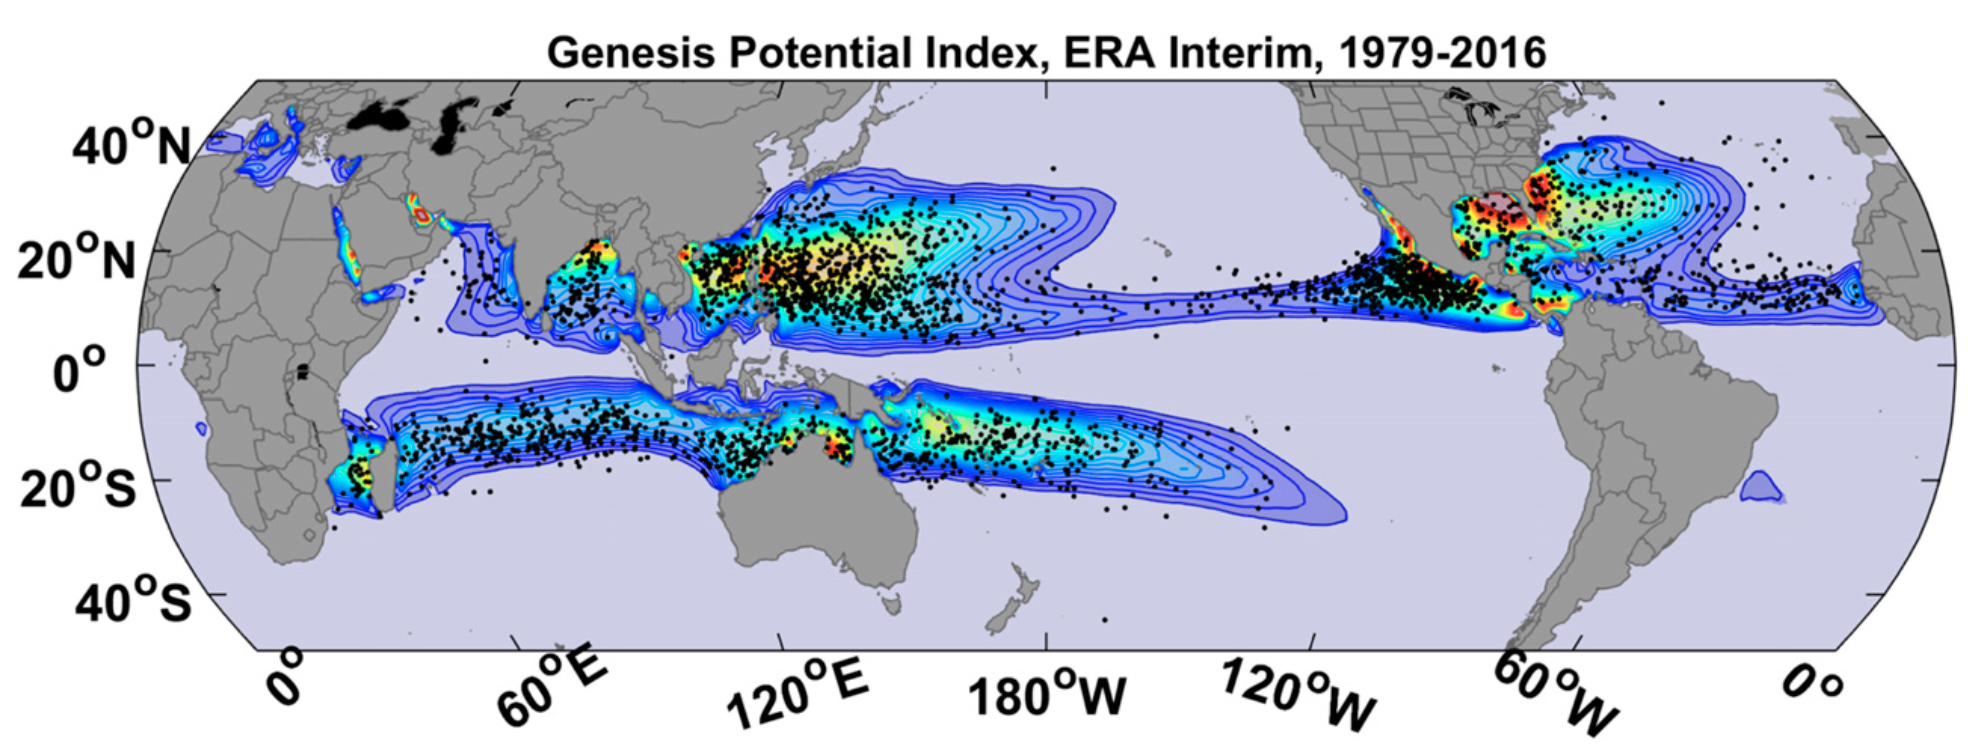
\includegraphics[width=\linewidth]{images/Genesis-Potential-Index.png}\\
\textit{Figure 15-15 from \cite{emanuel2018progress}.}
\caption{The annual maximum from Emanuel 2010~\cite{}. ERA-Interim data 1979-2016~\cite{berrisford2009era}.
The black dots show points recorded in tropical cyclone data~\cite{}.
}
\label{fig:genesis}
\end{figure*}
